% !TeX root = ./0-handout.tex

%details on counters; setting it to 0 prints everything with a roman I
%https://www.overleaf.com/learn/latex/Counters

%https://tex.stackexchange.com/questions/555149/how-do-i-change-the-frame-continuation-counter-from-roman-numerals-i-ii-iii

%\newcounter{mysection}
%\setcounter{mysection}{1}
%\arabic{mysection}
%\roman{subsection}

%\begin{itemize}[<+->] 
%\item<2-> % reveals second and keeps on page in subsequent frames
%\begin{itemize}[<2->] %does for a whole list of items


\setcounter{section}{-1} %sets section counter to 0. note that need to switch section counter from Roman to arabic for this to work! since no roman numeral for 0! %put this into preamble, i.e. file common.tex: \renewcommand\thesection{\arabic{section}}




\section{What are we Doing Here?}
%\subsection*{test}

\begin{frame}
%\large

\scriptsize{\tableofcontents}

\end{frame}

\subsection{Bureaucratic Basics}



%\subsection{First ordinals First: What is this class?}

\begin{frame}
  \frametitle{Zeroth ordinals First: Answering common questions!}
    
    \begin{itemize}[<+->] 
    \item The course materials on MITx is the CORE of the content, at least for the problem sets
    \item Hunt and the TAs will expect you to have read through this written material beforehand (eat your vegetables!)
    \item Watching the \textit{videos} on MITx is totally optional 
    \item Hunt will cover some technical basics in class, \\ model problem-solving (active learning woooooo), and \\ supplement with additional philosophical content that willl hopefully secure the ``Humanities'' in this HASS course. 
\item (The problem sets will be mainly technical)
\item \textbf{Sections are meeting this Friday}! \\ -- Join a section using Canvas sign-up tool!
    
  \end{itemize}
  
   \end{frame}

%\iffalse
\begin{frame}
  \frametitle{First ordinals Second: What is this class?}
  
  See the syllabus!!! See Canvas page! Enroll in \emph{MITx} page!
  
    \begin{itemize}[<+->] 
\item All course materials FREE on MITx: written text and videos 
        \item No required textbook, but if you cherish the printed word, Rayo's \textit{On the Brink of Paradox} is worth it.
    \item Problem Sets typically \emph{due Sundays 5pm}
    \item No extensions! Imagine that the PSet is really due on Friday or Saturday and we've \textit{already} given an extension to Sunday :D
   \item Scan to a pdf and submit on Canvas
   \item Hunt's office hours: after class on Thursday 12--1, 2--3
   %\item Hunt's office hours TBD based on when various reading groups are scheduled (but probs after class on Thursday 12--1, 2--3)
    \item 32D-962: 9th floor, Dreyfoos Wing (elevators nearest Vassar St.); turn RIGHT after entering Phil dept: office within an office 
\item[] (it's offices all the way down)
    
  \end{itemize}

  
  \end{frame}

\frame{\frametitle{Second (third?): Why come to Lecture?}
\large
\begin{itemize}[<+->] 

\item \textit{Intellectually}: We'll do philosophy! It'll be fun!

\item \textit{Spiritually}: You'll $<$3 it, or you can try to get me sacked! 

\item \textit{Instrumentally}: coming to 46\% of lectures accounts for 9\% of your grade! (12 lectures, out of 26 total)



%\item We'll cover the essential content, in a digestible manner \\ (helpful if you find it hard to make time to read)

\item We'll do practice problems! Often geared toward homework questions

\medskip

\item Although this is a problem-based course, I am hoping that you will acquire an appreciation for philosophy

\item (so that later in life, after you're a multi-millionaire hedge fund manager, you think about the little guy up there in the philosophy dept and write some \#\emph{PHAT} checks)

%\item You might gain some `insider information'

\bigskip

%\item This is a \emph{skills-based} course: \\ the goal is to learn how to \emph{do} logic, rather than to memorize or regurgitate facts about logic.

%\item Doing ample practice problems will be \emph{essential}!



\end{itemize}
}
  
  %\fi

\begin{frame}
\frametitle{Introducing: Our Stalwart TAs!}
%\large

  \begin{columns}
    \begin{column}{.3\textwidth}<1->
      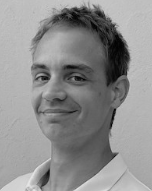
\includegraphics[height=.7\textheight]{../assets/philipp}
      
      Philipp Mayr!
    \end{column}
    \begin{column}{.27\textwidth}<2->
     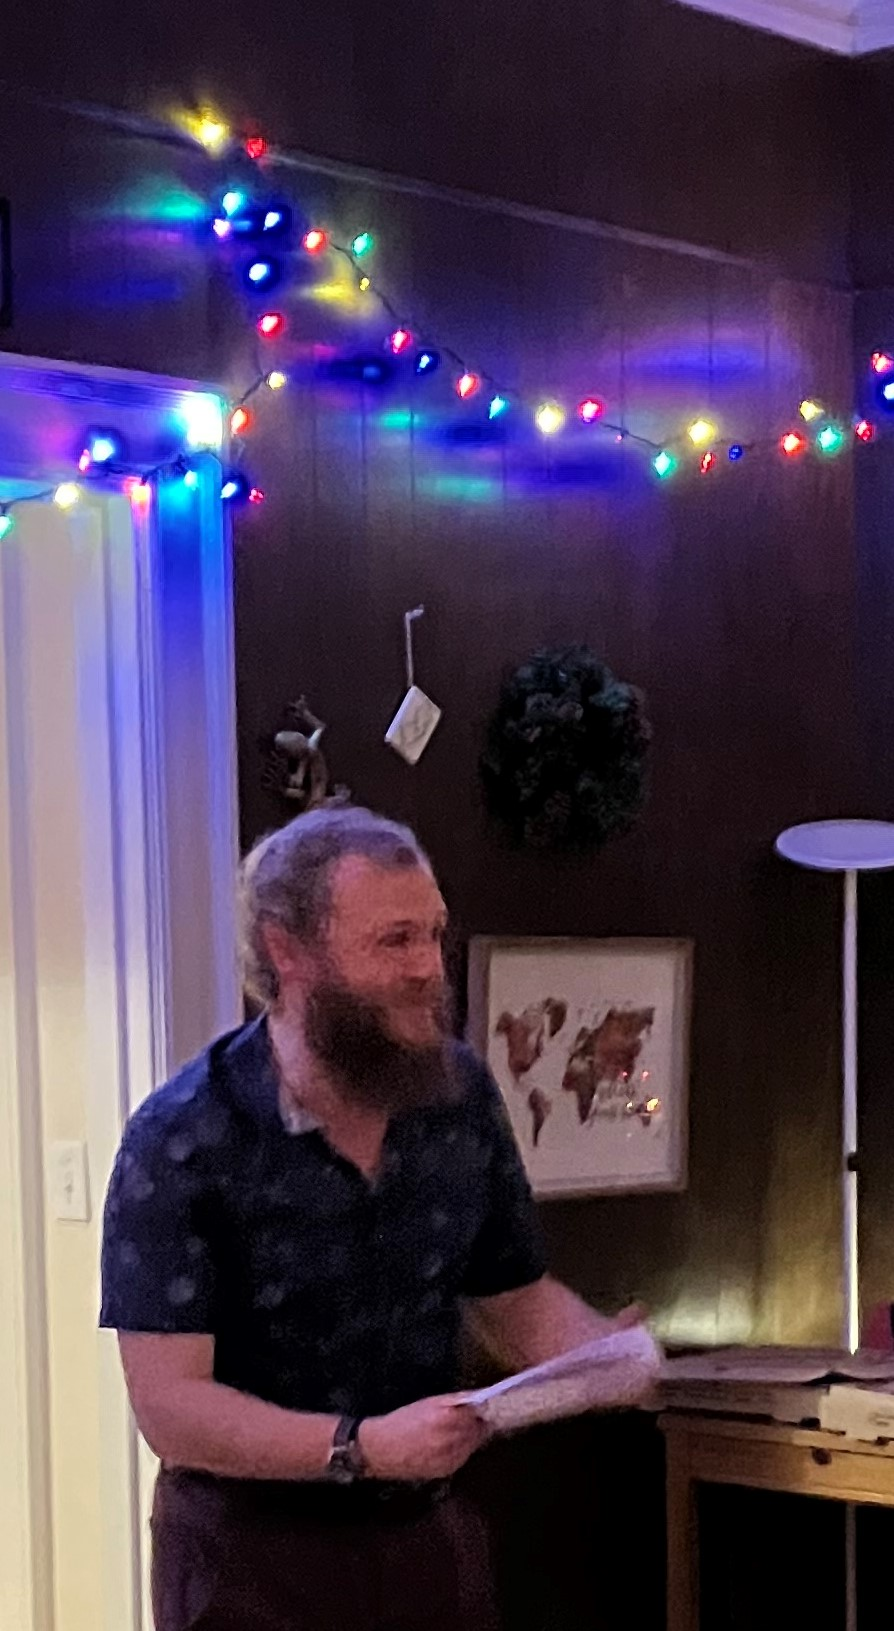
\includegraphics[height=.7\textheight]{../assets/gareth_cropped}
      
      Gareth Norman!
    \end{column}
 \begin{column}{.35\textwidth}<3->
     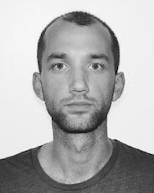
\includegraphics[height=.7\textheight]{../assets/pearson}
      
      Josh Pearson! (`Josh$_1$')
%\footnotesize{(`Josh$_1$')}
    \end{column}
  \end{columns}

\begin{itemize}[<+->]

\item Before Friday, please select a recitation section, using the Section Signup tool on Canvas

\item The three recitations are Friday 10, 11, and 12 (50 minutes each)
\end{itemize}
\end{frame}
  
  \begin{frame}
  \frametitle{Names and Quick Intros}
  
    \begin{itemize}[<+->]
    \item We're hoping that you'll feel completely comfortable in lecture and recitation
    \item It'll probably be easier to focus if you feel comfortable
    \item I find it helps to know some people to feel comfortable!
\item Let's meet some people!
\item Please introduce yourself to your two nearest neighbors: say your name, major, and one thing that brings you joy. 
  \end{itemize}
  
  \end{frame}

\subsection{What is Philosophy?}

\begin{frame}
\frametitle{A Few Conceptions of Philosophy}
%\large

\begin{itemize}[<+->]

\item Plz raise yo' hands to the roof if this is your first philosophy class

\item Aims at the \emph{T}ruth (with a capital `T')! (Plato; 427-347 B.C.E.)

\item Aims at reflective equilibrium (John Rawls; 1921--2002)

\item Aims at exploring logical space (Crispin Wright; 1942--\footnotesize{still kickin'!})

\item Aims at providing therapy for troubled minds \\ (Ludwig Wittgenstein; 1889--1951)

\item Notice that on all of these conceptions, philosophy aims at providing some kind of wisdom. So at least there's that :D

\end{itemize}
\end{frame}

\begin{frame}
\frametitle{Lessons from writer William Faulkner (1897--1962)}
%\large

\begin{itemize}[<+->]

\item Faulkner in his 1950 nobel prize speech: \\ We have ``forgotten the problems of \textit{the human heart in conflict with itself} which alone can make good writing because only that is worth writing about, worth the agony and the sweat."
%``The only thing worth writing about is the human heart in conflict with itself, regardless of genre"
%``the human heart in conflict with itself is the only thing worth writing about, regardless of the genre"
%Actual quote ``Because of this, the young man or woman writing today has forgotten the problems of the human heart in conflict with itself which alone can make good writing because only that is worth writing about, worth the agony and the sweat."

\item \emph{Upshot for us}: \textit{The intellect in conflict with itself is the only thing worth philosophizing about}

\item Our course will consider places of tension within modern mathematics, physics, decision theory, and logic 

\item If you are not already disturbed, you may become puzzled.
%like how i felt upon first hearing that there are reasons to be worried about infinity! had never occurred to me. i used infinity all the time! michael friedman talk in 2012 perhaps. 

\item Like Humpty Dumpty falling off the wall, it may be that all the philosophical horses won't be able to put you back together again 

\item We will seek to provide therapy 
\item[] (but only after convincing you that you really need therapy!)

\end{itemize}
\end{frame}

\begin{frame}
\frametitle{Of Pirates and Philosophers}
%\large

\begin{itemize}[<+->]

\item \emphz{Pirate's Mantra}: take what you can, give nothing back!

\item \emph{Philosopher's Mantra}: question everything, accept nothing!

\item Note well: there is a serious worry about becoming a troll

\item Strive to question sincerely \& deliberately, rather than reflexively

\end{itemize}
\end{frame}

\begin{frame}
\frametitle{Things Hunt is liable to forget to mention}
%\large

\begin{itemize}[<+->]

\item Please complete the Most Basic Factz survey on Canvas
\item[] It will function as attendance points for today (tricked ya!)
\item[] Please complete by this Saturday!

\item Feel free to join PSet partners!!! 
\item[] Groups will be auto-assigned every Friday

\item On Thursday we'll begin the philosophy prompt method of taking attendance (oooooooooooo ahhhhhhhhhhhhh)



\end{itemize}
\end{frame}

\subsection{To the syllabus!} 


\subsection{Philosophical Appraisals of Mathematics}

\begin{frame}
\frametitle{More Things Hunt is Liable to Forget!}
%\large

\begin{itemize}[<+->]

\item If you are on the waitlist and in class today, please let Hunt know after class and write your email (legibly) 

\item Misspoke last time about cheating-detection policy: if two people cheat and both report each other, they both lose 2 grade points! (better than being reported and losing 4!)

\item Review conceptions of philosophy from last time!


\end{itemize}
\end{frame}

\begin{frame}
%\frametitle{To Vindicate, Revise, or Reject?}
\frametitle{To Vindicate, Restrict, or Revise/Reject?}
%\large

\begin{itemize}[<+->]

\item A central choice point: \textit{what say you} about mathematics?

\item \emph{Vindication}: math is doing great! Keep this ship sailing!

\item \emph{Meh}: everyone stays aboard, but we're not exactly happy sailors

\item \emph{Restriction}: math is doing mostly fine, but we have some issues\dots. Someone's going overboard! 

\item \emph{Revision}: this ship is f$^{***}$ed; abandon ship!!! 
% Famous examples: folk psychology (churchlands); causation (russell)

\item Note that restriction and revision both involve \textit{rejecting} parts of classical math, to different extents. 

\item One true testament to the success of mathematics: \\ no one is trying to \emphz{eliminate} it, unlike other parts of our discourse 
\item[] (e.g. folk psychology, causation, astrology, witchcraft \& wizardry)

%\item This is a continuum, so the divisions between `revision' and `rejection' can be a bit blurry. 


\end{itemize}
\end{frame}



\begin{frame}
\frametitle{Ways of Vindicating}
%\large

\begin{itemize}[<+->]

\item \emph{Realism}:

\bi

\item \textit{Platonism}: mathematical objects and structures exist objectively and mind-independently outside the universe

\item \textit{Semantic realism}: mathematical claims are true objectively and mind-independently, in a non-deflationary sense. 

\ei

\bigskip

\item \emph{Formalism}: classical mathematics is a rule-governed game (like chess). The rules determine which inferences are permissible.

\item \emph{Logicism}: the permissible parts of math follow from the laws of logic (and we hope that this recovers all of mathematics!)

\item \emph{Structuralism}: mathematical entities exist as functional roles within a structure, similar to how the US president exists only relative to the US (\#LandoftheFree) 
% distinction between in re vs. ante rem structuralism.

% entities perform a functional role within a structure

%\item \emph{Inferentialism}:

%\item \emph{Expressivism}:

\end{itemize}
\end{frame}

\begin{frame}
\frametitle{Non-restrictive but NOT vindicatory}
%\large

\begin{itemize}[<+->]

\item \emph{Error Theory}: something is seriously amiss with the discourse of classical mathematics, but it is practically effective

\bi
\item \textit{Fictionalism}: mathematical entities are fictional, like our dearly beloved Sherlock Holmes. 
\item Mathematical claims are at most \textit{true in a fiction}. \\ None of these entities \textit{actually} exist.
\ei

\bigskip 

\item \emph{Quietism}: the mathematicians are doing what they are doing. Who are we to judge? 



\end{itemize}
\end{frame}

\begin{frame}
\frametitle{Ways of Restricting}
%\large

\begin{itemize}[<+->]

\item \emph{Naturalism}: preserve only those parts of math that are instrumentally valuable for physics or natural science. 
\item[] Reject unapplied parts, e.g. higher reaches of set theory 

\medskip 

\item \emph{Constructivism}: ``God made the integers, all else is the work of man" -- Leopold Kronecker (1823--1891)
%criticized Cantor as corrupting the youth!!!

\bi
\item TL;DR: stick to what's computable, son!
\ei

\medskip 

\item \emph{Finitism}: if it ain't finite, it doesn't count. 
\item[] Still allows for computations that could take arbitrarily long but still finite length (e.g. longer than anything computable within the time span in which a universe supports life)

\end{itemize}
\end{frame}

\begin{frame}
\frametitle{Ways of Revising (classical mathematics)}
%\large

\begin{itemize}[<+->]

\item \emph{Intuitionism}: the mind creates mathematics, relying primitively on the notion of time's passing. -- L.E.J. Brouwer (1881--1966)
\bi
\item Comes into conflict with classical mathematics regarding the proper conception of the real numbers and the continuum. 
\item So intuitionism is NOT a restriction of classical math
\ei

%%``Brouwer’s second act of intuitionism gives rise to choice sequences, that provide certain infinite sets with properties that are unacceptable from a classical point of view. A choice sequence is an infinite sequence of numbers (or finite objects) created by the free will. The sequence could be determined by a law or algorithm, such as the sequence consisting of only zeros, or of the prime numbers in increasing order, in which case we speak of a lawlike sequence, or it could not be subject to any law, in which case it is called lawless."

%%sense in which intuitionism is diff from constructivism (but I thought intuitionisitic logic IS a restriction of classical logic?):
%``intuitionism strongly deviates from classical mathematics in the conception of the continuum, which in the former setting has the property that all total functions on it are continuous. Thus, unlike several other theories of constructive mathematics, intuitionism is not a restriction of classical reasoning"
%https://plato.stanford.edu/entries/intuitionism/
%Brouwer history sounds very interesting: ``the most famous one being the conflict with David Hilbert, which eventually led to Brouwer’s expulsion from the board of the Mathematische Annalen. This conflict was part of the Grundlagenstreit that shook the mathematical society at the beginning of the 20th century and that emerged as a result of the appearance of paradoxes and highly nonconstructive proofs in mathematics. "

%%``intuitionism differs from Platonism and formalism, because neither does it assume a mathematical reality outside of us, nor does it hold that mathematics is a play with symbols according to certain fixed rules. " formalism sounds similar to expressivism/norms in some regard. 

%% ``The distinction between intuitionism and other constructive views on mathematics according to which mathematical objects and arguments should be computable, lies in the freedom that the second act allows in the construction of infinite sequences. Indeed, as will be explained below, the mathematical implications of the second act of intuitionism contradict classical mathematics, and therefore do not hold in most constructive theories, since these are in general part of classical mathematics"

\bigskip

\item \emph{Ultra-finitism}:  if it ain't \textit{small enough}, it's bullsh$^{**}$. 
\item[] (a philosophy completely against ``too big to fail")

\bigskip

\item \emph{Anti-democracy}: Defunding public school education in America

\end{itemize}
\end{frame}

\begin{frame}
\frametitle{A Philosophy Prompt (\#1)}
%\large

\begin{itemize}[<+->]

\item On your bespoke little sheet of paper, write at least five non-trivial sentences in response to the following:

\item Presently, are you disposed to defend an attitude of vindication, restriction, or revision when it comes to contemporary mathematics? 
\item[] -- To what extent have you ever thought about this kind of philosophical question?
\item[] -- To spice things up, feel free to comment on \emph{infinity}, \emph{non-constructive proofs}, or the \emph{axiom of choice}. 

\item Throughout the course, we'll be cultivating a \textit{growth mindset}, so no need to become attached to your current disposition(s)!



\end{itemize}
\end{frame}

\iffalse %*****************************************************

%\subsection{Time to get Injected!}
\subsection{Onto Injections! (They go both ways)}

\begin{frame}
\frametitle{Basics of Functions}
%\large

\begin{itemize}[<+->]

\item Consider a function $f$ (a.k.a. `map') from a \emph{domain} set $A$ to a \emphz{range} set $B$. We denote this as ``$f: A \rightarrow B$". 

\item To be \emph{well-defined}, EVERY element of $A$ must be mapped by $f$ to exactly one (not necessarily distinct) element of $B$

\item[] $\forall a \in A, \exists ! b \in B$ such that $f(a) = b$

\item[] (Note that the order of the quantifier matters a great deal: $\exists ! b \in B$ s.t. $\forall a \in A$,  $f(a) = b$ is a horizontal line if $A = B = \mathbb{R}$)

\item Note that the \emph{image} of $f$, ``$f(A)$", need not equal the entire range $B$: in general, $f(A) \subseteq B$

\item When the image equals $B$, we say that the function is \emph{onto}, a.k.a. ``a \emph{surjection}"

\end{itemize}
\end{frame}

\begin{frame}
\frametitle{Something we are all liable to forget to do!}
%\large

\begin{itemize}[<+->]

\item If you are asked to prove something that involves constructing a function $f: A \rightarrow B$, you ought to first show that the function is \emph{well-defined}:

\item i.e. that each element of the domain is sent to a unique element of the range

\item Basically, given an arbitrary $a \in A$, argue (i) that $f(a) \in B$ and that (ii) if there are $b \neq b'$ in $B$ such that both $b = f(a)$ and $b' = f(a)$ then we have a contradiction. 

\item Often, it is so seemingly `obvious' that a function is well-defined, that explicitly proving this will seem tedious and annoying.

\item[] \textit{spoiler}: philosophers have a tendency to be tedious ;) 

%\item Note that every element in the domain is sent to a single element in the range

% Note that the motivation for requiring functions to be well-defined is actually kind of interesting. You need different representatives of the same number to be sent to the same value, e.g. f(0.5) to equal f(1/2) and f(1) to equal f(0.9999999999) 


\end{itemize}
\end{frame}

\begin{frame}
\frametitle{Injections (ivermectin anyone?)}
%\large

\begin{itemize}[<+->]

\item \emph{Injection}: $\forall x, y \in A$, if $f(x) = f(y)$, then $x = y$.
\item[] Intuitive gloss: each element $a$ of the domain $A$ is mapped to a unique element $b$ of the range $B$. 
\item[] -- If $a$ is mapped to $b$, then NO OTHER $x \in A$ is mapped to $b$
\item[] --Monogamous heterosexual norm-core marriages define an injection from monogamous-married men to women. 

\item  \emph{How to prove a function is injective}: consider two \textit{arbitrary} elements $x, y \in A$. Assume for the sake of argument that $f(x) = f(y)$. Proceed to show that $x=y$ (e.g. via algebra).

\item \emphz{How to prove a function is NOT injective}: \\ provide a concrete counterexample. i.e. identify two $x, y \in A$ such that $f(x) = f(y)$ but $x \neq y$.
\item[] e.g. $f(x) = x^2$

\end{itemize}
\end{frame}

\begin{frame}
\frametitle{Some Practice with Injections \& Surjections}
%\large

\begin{itemize}[<+->]

\item For each function below, determine whether it is (a) injective and (b) surjective:

\item Recall: Natural numbers $\mathbb{N} := \{ \mathbf{0}, 1, 2, \dots \}$ (we include zero!)

\item Integers $\mathbb{Z} := \{ \dots, -2, -1, 0, 1, 2, \dots \}$

\end{itemize}

\begin{enumerate}[<+->]

\item $f(x) = x+1$ where $f: \mathbb{N} \rightarrow \mathbb{N}$
%injective but not surjective because no natural number hits zero 

\item $f(x) = x^2$ where $f: \{ 1, 2, 3, \dots, 10 \} \rightarrow \{ 1, 2, \dots, 100 \}$
%injection but not surjection. e.g. 2 is not the square of anything in the domain 

\item $f(x) = x^2$ where $f: \{ -5, -4, \dots, -1, 0, 1, 2, \dots, 5\} \rightarrow \{ 0, 1, 4, 9, 16, 25 \}$

\item $f(x) = x^3$ where $f: \mathbb{Z} \rightarrow \mathbb{R}$
%injective but NOT surjective, e.g. no integer hits $\sqrt{2}$ or $\pi$ 

\end{enumerate}
\end{frame}

\begin{frame}
\frametitle{Bijections: injective surjections! (``1-to-1 and onto")}
%\large

\begin{itemize}[<+->]

\item A function $f: A \rightarrow B$ is a \emph{bijection} just in case it is \\ both (i) injective and (ii) surjective

\item[] e.g. $f(x) = x$ from $\mathbb{R}$ to $\mathbb{R}$ is a bijection 

\item \emph{To prove a bijection}: method one: construct it! 
\item[] Show that the purported bijection $f$ is (0) well-defined, \\ (i) injective, and (ii) surjective

\item \emphz{Method Two}: use the Cantor-Schroeder-Bernstein Theorem:
\item[] (i) Construct an explicit injection in one direction, \\ then (ii) an injection in the other direction
\item[] -- Remember that injections don't have to be onto, so this can simplify things (e.g. if $A \subset B$, you can use the identity function)


\end{itemize}
\end{frame}


\begin{frame}
\frametitle{Some practice with Cardinality}
%\large
Between which of the following sets is it possible to construct a bijection (i.e. which sets have the same cardinality)?

\begin{enumerate}[<+->]

\item $\mathbb{N}$ and $\mathbb{Z}$ ? 

\item $\mathbb{Q}$ and the reals between 0 and 1, i.e. $(0, 1)$ ?

\item $\mathbb{R}$ and $\mathscr{P}(\mathbb{R})$ ? 

\end{enumerate}

\end{frame}


\begin{frame}
\frametitle{Some practice with Bijections}
%\large

Recall: a bijection is an injective surjection 

\begin{enumerate}[<+->]



\item Construct a bijection from the integers to the natural numbers, $f: \mathbb{Z} \rightarrow \mathbb{N}$ (helps with a PSet \#1 problem)
% send the positive integers to the evens: 2n; send the negative integers to the odds: -2n -1

\item Construct a bijection from $\mathbb{N}$ to the set of prime numbers \\ (you may assume that given a finite set of primes, there is a \textit{smallest} prime number greater than every prime in that set)
%2022 Pset 1, number 7b; which I am changing to construct injection from set of integers to set of prime numbers. 

\item Argue that there is a bijection from $\mathbb{N}$ to $\set{\seq{n,m} : n,m \in \mathbb{N}}$, which is the set of pairs of natural numbers

\item Is there a bijection between $\mathbb{N}$ and the set $\{x : x$ is a function from $\mathbb{N}$ to the set $\{1, 2, 3, 4 \} \}$? 
% Analog of the Homer question involving earth, sun, moon

%\item Now a homework question! Construct a bijection from the set of integers to the set of prime numbers

%\item Construct a bijection from the set of prime numbers to the set of integers 

\end{enumerate}
\end{frame}



%\iffalse %************************************************************************


\subsection{Puzzles about `Size'}
%could call this size-matters 

% % Josh read the following one**********************************************************
%https://en.wikipedia.org/wiki/Controversy_over_Cantor%27s_theory

\begin{frame}
\frametitle{Two Conceptions of `Size'}
%\large

\begin{itemize}[<+->]

\item \emphz{Proper Subset Principle}:

\item \emph{Bijection Principle}: 

\item For finite sets, these principles agree, but they disagree for infinite sets

\end{itemize}
\end{frame}

\begin{frame}
\frametitle{Which Conception of Size should we Privilege?}
%\large

\begin{itemize}[<+->]

\item \emphz{Proper Subset Principle}:
\bi
\item accords better with our pre-theoretical intuitions

\item Intuitively, there are more rational numbers than natural numbers, since $\mathbb{N} \subset \mathbb{Q}$

\item Con: is mathematically sterile or `uninteresting' for infinite sets

\ei

\item \emph{Bijection Principle}:
\bi

\item Is mathematically fruitful! 

\item Aside: what is fruitfulness in mathematics? \\ -- What does it mean for a bit of mathematics to be `interesting'?

\item Con: leads to some pretty crazy sounding claims, e.g. that the interval $[0, 1]$ has the same size as $\mathbb{R}$, even though clearly $[0,1]$ is a very small `part' of the interval $(-\infty, \infty)$

\ei

\end{itemize}
\end{frame}

\begin{frame}
\frametitle{Finitism: privilege subset principle}
%\large

\begin{itemize}[<+->]

\item Weyl against Cantor's set theory:

\begin{quote}
classical logic was abstracted from the mathematics of finite sets and their subsets.\dots Forgetful of this limited origin, one afterwards mistook that logic for something above and prior to all mathematics, and finally applied it, without justification, to the mathematics of infinite sets. This is the Fall and original sin of [Cantor's] set theory" -- 1946
\end{quote}
%from Weyl, Hermann (1946), "Mathematics and logic: A brief survey serving as a preface to a review of The Philosophy of Bertrand Russell", American Mathematical Monthly, vol. 53, pp. 2–13,

\end{itemize}
\end{frame}

\begin{frame}
\frametitle{Why not Both?}
%\large

\begin{itemize}[<+->]

\item We could just introduce two different words, e.g. \emphz{size}$_{subset}$ and \emph{size}$_{bijection}$

\item No problem as long as we never equivocate, i.e. substitute one meaning of `size' for the other in a single argument

\item In practice, this is what we do: we talk about the subset relation `$\subset$' and also ``cardinality" `$\abs{S}$', which tracks the existence of bijections

\end{itemize}
\end{frame}

\begin{frame}
\frametitle{A Philosophy Prompt \#2}
%\large

\begin{itemize}[<+->]

\item You come home from math class one day and are super pumped to tell your parents, siblings, mailperson, and anyone willing to listen a MIND-BLOWING FACT: \textit{there are as many even numbers as odd and even numbers together}!

\item For those willing to listen, they tell you that you must be out of your god d*** mind: clearly, there are more natural numbers, since the evens are a proper subset of the natural numbers. 

\item Presently, how are you disposed to respond to your interlocutor?




\end{itemize}
\end{frame}

\begin{frame}
\frametitle{Some Possible Responses}
%\large

\begin{itemize}[<+->]

\item \textit{Hold your ground}: you're the one in the math class after all! Your layperson interlocutor doesn't know what's up!

\item \textit{Reject}: agree with your interlocutor that the mathematicians are up to something pretty strange. 

\item \textit{A therapeutic response}: you learned a technical sense of `size' in your math class that tracks the existence of bijections. 
\bi
\item You're basically just saying that there is a bijection between the even numbers and the naturals. 
\item That is interesting, but not nearly as cool sounding as saying that the evens have the same \emphz{size}$_{subset}$ as the naturals, which is probably how your interlocutor understood you.
\ei

\end{itemize}
\end{frame}



\subsection{Burali--Forti Paradox}

\begin{frame}
\frametitle{Burali--Forti Paradox}
%\large

\begin{itemize}[<+->]

\item We keep talking about the ordinals, but we can prove that there cannot exist a set of all ordinal numbers

\item In general, there can be no such thing as the set of all sets. Such a set would have to be a member of itself, and hence fail to contain every set.
%https://en.wikipedia.org/wiki/Absolute_Infinite


\end{itemize}
\end{frame}

\begin{frame}
\frametitle{Resolution in Zermelo's Set Theory}
%\large

\begin{itemize}[<+->]

\item Here's one solution: declare it impermissible to form a set from an arbitrary property (reject ``unrestricted comprehension")

\item Axiom of separation/comprehension: it is permissible to form a set of objects that have a given property provided that they belong to a given set. 

\item i.e. any definable subclass of a set is itself a set 
%https://en.wikipedia.org/wiki/Axiom_schema_of_specification

\item But if a class of individuals exists, why can't we in general form a \textit{set}??? If there is no set, might we worry that some of the individuals in fact do not exist?

\item Does it start to feel like we are playing a game rather than surveying Platonic space?

\item Alternatively, given that our meta-language contains predicates that refer to classes that are not sets within our theory, might we worry that our theory is \textit{missing something}

% Our metalanguage contains predicates that do not refer to any sets within the theory 
%https://en.wikipedia.org/wiki/Absolute_Infinite

\end{itemize}
\end{frame}




\fi %********************************************************************************



\iffalse


\subsection{Arguments and validity}

\frame{\frametitle{Causes vs. (normative) Reasons for belief}
\large
\begin{itemize}

\item \emph{Causes of belief}: why you actually believe something

\begin{itemize}[<2->]

\item Attacked by cat at age 8: causes you to believe `cats are dangerous'

\item These are \textit{descriptive} reasons for belief

\item Often these are not rationally compelling reasons

\end{itemize} 

\item<3->  \emph{Reasons for belief}: why you \textit{ought} to believe something

\begin{itemize}[<4->]

\item Empirical data on cat attacks per capita  

\item These are \textit{normative} reasons for belief

\item Logic aims to characterize the structure of such reasons, when organized into \textit{arguments}
% Tappenden: arguments are premises supporting conclusions that logically purport to give reasons for belief (not in the sense of causes for belief)

\end{itemize}

\end{itemize}
}

\frame{\frametitle{Rhetorically vs. Logically Good Arguments}
\large
\begin{itemize}

\item \emph{Rhetorically good argument}: argument that actually persuades listeners

\begin{itemize}[<2->]

\item Might be \textit{descriptively good}, while being logically awful

\item Might rely solely on emotional tricks or rhetoric

\item Anecdotes: ``my friend got a blood clot from the Johnson \& Johnson Covid vaccine. Therefore, avoid this vaccine!''  

\item A plane recently crashed: I better drive!

\end{itemize}

\item<3->  \emph{Logically good arguments}: arguments that \textit{ought} to persuade listeners, if they were rational

\begin{itemize}[<4->]

\item Such arguments might be descriptively pretty unpersuasive!

\item Comparative analysis of risk of blood clots from Janssen vaccine vs. risk of negative Covid health outcome 

\item Comparative analysis of plane crashes vs. car crashes

\end{itemize}



\end{itemize}
}

\begin{frame}
  \frametitle{An easy puzzle}

  \begin{block}{Where does Sanjeev live?}
  Sanjeev lives in Chicago or in Erie.\\
  Sanjeev doesn't live in Erie.
  \end{block}

  \begin{itemize}
    \item<2>[A:] Obviously, in Chicago.
  \end{itemize}

\end{frame}

\begin{frame}
  \frametitle{Arguments and sentences}

  \begin{block}{Argument 1}
  Sanjeev lives in Chicago or in Erie.\\
  Sanjeev doesn't live in Erie.\\
  Therefore, Sanjeev lives in Chicago.
  \end{block}

  \begin{itemize}[<+->]
  \item Such an argument consists of (declarative) \emph{sentences}.
  \item Declarative sentences are the kinds that can be \emph{true} or \emph{false}.
  \item ``Therefore'' ($\therefore$) indicates that the last sentence (supposedly)
  \emph{follows from} the first two.
  \item The last sentence is called the \emph{conclusion}.
  \item The others are called the \emph{premises}.
  \end{itemize}

\end{frame}

%JRH: would be better to contrest MP with affirming the consequent; e.g. Angela Merkel example 

\begin{frame}
  \frametitle{Valid and invalid arguments}

  \begin{block}{Argument 2}
  Mandy enjoys skiing or hiking (or both).\\
  Mandy doesn't enjoy hiking.\\
  $\therefore$ Mandy enjoys skiing.
  \end{block}

  \begin{block}{Argument 3}
  Mandy enjoys skiing or hiking (or both).\\
  Mandy enjoys skiing.\\
  $\therefore$ Mandy doesn't enjoy hiking.
  \end{block}

  What's the difference?

  \note[itemize]{
    \begin{itemize}
    \item Arg 2 is like argument 1
    \item Think-pair-share argument 2
    \item Depending on result of experiment/agreement talk about
    inclusive/exclusive
    \item Argument 2 is valid if the ``or'' is exclusive.
    \end{itemize}
  }
\end{frame}


\begin{frame}
  \frametitle{(Deductive) Validity}

  \begin{definition}<1->
  An argument is (deductively) \emph{valid} if there is no case where all its
  premises are true and the conclusion is false.
  \end{definition}

  \begin{definition}<2->
  An argument is \emph{invalid} if there is at least one case where
  all its premises are true and the conclusion is false (i.e., if it
  is not valid).
  \end{definition}

  \begin{definition}<3->
  A \emph{case} is some hypothetical scenario that makes each sentence
  in an argument either true or false.
  \end{definition}
\end{frame}

\begin{frame}
  \frametitle{Argument 2 is valid}

  \begin{block}{Argument 2}
  Mandy enjoys skiing or hiking.\\
  Mandy doesn't enjoy hiking.\\
  $\therefore$ Mandy enjoys skiing.
  \end{block}

Argument 2 is \emph{valid}: whenever the premises are
true, the conclusion is also true.

\end{frame}

\begin{frame}
  \frametitle{Argument 3 is not valid}

  \begin{block}{Argument 3}
  Mandy enjoys skiing or hiking.\\
  Mandy enjoys skiing.\\
  $\therefore$ Mandy doesn't enjoy hiking.
  \end{block}

  Argument 3 is \emph{invalid}: there is a possible case where the
  premises are true and the conclusion isn't (Mandy enjoys both skiing
  and hiking).

\end{frame}

\begin{frame}
  \frametitle{A harder puzzle}

  \begin{block}{Where does Sarah live?}
  Sarah lives in Chicago or Erie.\\
  Amir lives in Chicago unless he enjoys hiking.\\
  If Amir lives in Chicago, Sarah doesn't.\\
  Neither Sarah nor Amir enjoy hiking.
  \end{block}

\end{frame}

\subsection{Cases and determining validity}

\begin{frame}
  \frametitle{Validity}

  \begin{definition}
  An argument is \emph{valid} if there is no case where all its
  premises are true and the conclusion is false.
  \end{definition}

  \begin{definition}
  An argument is \emph{invalid} if there is at least one case where
  all its premises are true and the conclusion is false (i.e., if it
  is not valid).
  \end{definition}
\end{frame}

\begin{frame}{Cases}
  
\begin{definition}
  A \emph{case} is some hypothetical scenario that makes each sentence
  in an argument either true or false.
\end{definition}

\begin{itemize}[<+->]
  \item E.g., imagine you have a friend, her name is Mandy, she loves
  hiking but hates skiing.
  \item That's a case where ``Mandy enjoys hiking or skiing'' is true.
  \item Some cases can be imagined even though they never happen IRL, e.g,
  ``It is raining and the skies are clear.''
  \item Some things you can't imagine, e.g.,
  ``There is a blizzard but there is no wind.''
\end{itemize}

\end{frame}

\begin{frame}
  \frametitle{Determining validity}

  \begin{itemize}[<+->]
    \item Imagine a case where the conclusion is false.
    \item Are the premises true? You're done: invalid.
    \item Otherwise, change or expand the case to make them true
    (without making the conclusion also true).
    \item Can't? (Probably) valid.
  \end{itemize}

  \uncover<5->{OR}

  \begin{itemize}[<+->]
    \item Imagine a case where all premises are true.
    \item Is the conclusion false? You're done: invalid.
    \item Otherwise, change or expand the case to make it false
    (without making the premises false).
    \item Can't? (Probably) valid.
  \end{itemize}
\end{frame}

\begin{frame}{Deductively Valid?}
  \begin{earg}
    \item[] Some rodents have bushy tails.
    \item[] All squirrels are rodents.
    \item[\therefore] Some squirrels have bushy tails.
  \end{earg}
\pause
  \begin{itemize}[<+->]
    \item Imagine squirrels evolving so that they no longer have bushy
    tails. Then conclusion is false.
    \item But premises still true:
    \begin{itemize}[<+->]
      \item Imagine chinchillas still have bushy tails.
      \item Imagine also that squirrels have not evolved too
      much---they are still rodents.
    \end{itemize}
  \end{itemize}
\end{frame}

\begin{frame}{Valid?}
  \begin{earg}
    \item[] All rodents have bushy tails.
    \item[] All squirrels are rodents.
    \item[\therefore] All squirrels have bushy tails.
  \end{earg}
\pause
  \begin{itemize}[<+->]
    \item If it were invalid, you'd have a case that makes the
    conclusion false: some squirrels without bushy tails.
    \item They would have to be rodents still (otherwise premise 2 false).
    \item And that would require that they have bushy tails (otherwise premise 1 false).
  \end{itemize}
\end{frame}

\subsection{Other logical notions}

\begin{frame}
  \frametitle{Logical Consistency}

  \begin{definition}
  Sentences are (logically) \emph{consistent} if there is a case where they
  are all true. \\ $\bullet$ also called `jointly possible' or `satisfiable' 
  \end{definition}

  \begin{definition}
    Sentences are (logically) \emph{inconsistent} if there is no case where they
    are all true. \\ $\bullet$ also called `jointly impossible' or `unsatisfiable' 
    \end{definition}
\end{frame}


\begin{frame}
  \frametitle{Consistent?}
  \begin{earg}
    \item[] Some carnivores have bushy tails.
    \item[] All carnivores are mammals. 
    \item[] No mammals have bushy tails.
  \end{earg}

  \begin{itemize}
    \item<2> No case makes them all true at the same time, so
    \emph{inconsistent}.
  \end{itemize}
\end{frame}

\begin{frame}
  \frametitle{Valid?}
  \begin{earg}
    \item[] Some carnivores have bushy tails.
    \item[] All carnivores are mammals. 
    \item[] No mammals have bushy tails.
    \item[\therefore] All birds are carnivores. 
  \end{earg}

  \pause

  \begin{itemize}[<+->]
    \item The premises cannot all be true in the same case, so inconsistent.
    \item So: no case makes all the premises true.
    \item So also: no case makes the premises true and the conclusion false.
    \item \emph{Arguments with inconsistent premises are automatically
    valid}, regardless of what the conclusion is.
  \end{itemize}
\end{frame}

\begin{frame}{Tautology (logically necessary)}

  \begin{definition}
    A sentence is a \emph{tautology} if there is no case where
    it is false. \\ $\bullet$ also called a `necessary truth' or `truth-functionally true'
    \end{definition}
\pause
    \begin{itemize}[<+->]
      \item If it's snowing, then it's snowing.
      \item Every fawn is a deer.
      \item The number 5 is prime.
\item It's not the case that I am standing and that I am not standing. \\ (`\textit{Law of Non-Contradiction}')
      %\item Physical objects are extended.
    \end{itemize}
\end{frame}

\begin{frame}{Tautology}
    What can you say about an argument where the conclusion is a
    tautology? 
\pause
\begin{itemize}[<+->]
  \item If the conclusion is a tautology, there is no case where
  it is false.
  \item So there is no case where both (1) it is false and (2) the premises of the
  argument are all true.
  \item $\Rightarrow$ \emph{Arguments with tautologies as conclusions are
  automatically valid}, regardless of what the premises are.
\end{itemize}
  \end{frame}

\begin{frame}
  \frametitle{Logical equivalence}

  \begin{definition}
  Two sentences are (logically) \emph{equivalent} if there is no case where one is
  true and the other is false.
  \end{definition}

  \begin{itemize}[<+->]
    \item What can you say about an argument where one of the premises
    is equivalent to the conclusion? Is it automatically valid?
    \item Can you have two equivalent sentences that are inconsistent?
  \end{itemize}

\end{frame}


\subsection{What are we going to learn? \\ And why?}

\begin{frame}
  \frametitle{What is logic?}

  \begin{itemize}[<+->]
  \item \emph{Logic is the science of what follows from what.}
  \item Sometimes a conclusion follows from the premises, sometimes it
  does not:
  \begin{itemize}[<+->]
    \item Mandy lives in Chicago.\\ Everyone who lives in Chicago likes hiking.\\
    $\therefore$ Mandy likes hiking.
    \item Mandy lives in Chicago.\\ Everyone who likes hiking lives in Chicago.\\
    $\therefore$ Mandy likes hiking.
    \end{itemize}
  \item Logic investigates what makes the first argument \emph{valid}
    and the second \emph{invalid}.
  \end{itemize}
\end{frame}

\begin{frame}
  \frametitle{What is formal logic?}

  \begin{itemize}[<+->]
  \item Studies logical properties of \emph{formal languages} (SL and
  QL, not English).
    \begin{itemize}[<+->]
    \item Logical consequence (what follows from what?)
    \item Logical consistency (when do sentences contradict one another?)
    \end{itemize}
  \item Expressive power (what can be expressed in a given formal
  language, and how?)
  \item Formal models (mathematical structures described by formal language)
  \item Inference and proof systems (how can it be proved that something
  follows from something else?)
  \item Meta-logical properties of logical systems
  \end{itemize}
\end{frame}

\begin{frame}
  \frametitle{Plan for the course}

  \begin{itemize}[<+->]
  \item Sentential Logic (SL), aka Truth-functional logic
    \begin{itemize}[<+->]
    \item Symbolization in the formal language of SL ($H, \lor,
    \land, \to, \lnot$)
    \item Testing for validity: truth-tables and TREES! 
    \item Proofs in natural deduction
    \end{itemize}
  \item Quantifier Logic (QL), aka First-order logic 
    \begin{itemize}[<+->]
    \item More fine-grained symbolization ($E(m,h)$, $\forall$
    `every', $\exists$ `some', $=$)
    \item Semantics: interpretations
    \item Proofs in natural deduction
    \end{itemize}
  \item Metalogic (sprinkled in Unit 1 as well!): 
 \begin{itemize}[<+->]
\item Soundness \& Completeness of our deduction systems
\item Compactness
\item Expressive completeness, normal forms
  \end{itemize}
  \end{itemize}
\end{frame}

\begin{frame}
  \frametitle{What is logic good for? (Philosophy)}

  \begin{itemize}[<+->]
  \item Logic originates in philosophy (e.g. Aristotle); \\ traditionally considered a sub-discipline of philosophy.
  \item Valid arguments are critical in philosophical research.
  \item Formal tools of logic are useful for making various philosophical
  notions precise, e.g.,
    \begin{itemize}[<+->]
    \item Possibility and necessity
    \item Time
    \item Composition and parthood (mereology)
    \item Moral obligation and permissibility
    \item Belief and knowledge
    \end{itemize}
  \item Logic applies to the semantics of natural language \\ (philosophy of
  language, linguistics).
  \end{itemize}
\end{frame}

\begin{frame}
  \frametitle{What is logic good for? (Mathematics)}

  \begin{itemize}[<+->]
  \item Formal logic was developed largely in a quest for the foundations of
  mathematics (19th century).
  \item Logical systems provide precise foundational framework for
  mathematics:
    \begin{itemize}[<+->]
    \item Axiomatic systems (e.g, geometry)
    \item Algebraic structures (e.g., groups)
    \item Set theory (e.g, Zermelo-Fraenkel with Choice)
    \end{itemize}
  \item Precision
    \begin{itemize}[<+->]
    \item Formal language makes claims more precise.
    \item Formal structures can point to alternatives, unveil gaps in proofs.
    \item Formal proof systems make proofs rigorous.
    \item Formal proofs make mechanical \emph{proof checking} and \emph{proof search} possible.
    \end{itemize}
  \end{itemize}

\end{frame}


\begin{frame}
  \frametitle{What is logic good for? (Computer Science)}

  \begin{itemize}[<+->]
    \item Computer science deals with lots of formal languages.
    \item Logic is a good example of how to set up and use formal languages.
    \item `Logic : Computer Science' $=$ `Calculus : Natural Science'
    \item Applications of logical systems in CS are numerous:
  \begin{itemize}[<+->]
  \item Combinational logic circuits
  \item Database query languages
  \item Logic programming
  \item Knowledge representation
  \item Automated reasoning
  \item Formal specification and verification (of programs, of hardware designs)
  \item Theoretical computer science (theory of computational
  complexity, semantics of programming languages)
 \end{itemize}
\end{itemize}

\end{frame}

\subsection{Symbolization and SL}

\begin{frame}
  \frametitle{Validity in virtue of form}

  \begin{block}<1->{Argument 1}
  Sanjeev lives in Chicago or Erie.\\
  Sanjeev doesn't live in Erie.\\
  $\therefore$ Sanjeev lives in Chicago.
  \end{block}

  \begin{block}<1->{Argument 2}
  Mandy enjoys skiing or hiking.\\
  Mandy doesn't enjoy hiking.\\
  $\therefore$ Mandy enjoys skiing.
  \end{block}

  \begin{block}<2>{Form of arguments 1 \& 2}
  $X$ or $Y$.\\
  Not $Y$.\\
  $\therefore$ $X$.
  \end{block}

\end{frame}

\begin{frame}
  \frametitle{Some valid argument forms}

  \begin{block}{Disjunctive syllogism}
  $X$ or $Y$.\\
  Not $Y$.\\
  $\therefore\ X.$
  \end{block}

  \begin{block}{Modus ponens}
  If $X$ then $Y$.\\
  $X$.\\
  $\therefore\ Y.$
  \end{block}

  \begin{block}{Hypothetical syllogism}
  If $X$ then $Y$.\\
  If $Y$ then $Z$.\\
  $\therefore$ If $X$ then $Z$.
  \end{block}
\end{frame}

\begin{frame}
  \frametitle{Symbolizing arguments}

  \begin{block}{Symbolization key}
  $S$: Mandy enjoys skiing\\
  $H$: Mandy enjoys hiking
  \end{block}

  \begin{block}{Argument 2}
    \begin{tabular}{@{}l@{}l@{}}
      Mandy enjoys skiing or Mandy enjoys hiking.  & \ \emph{$(S \lor H)$}\\
      Not: Mandy enjoy hiking. & \emph{$\lnot H$}\\
      $\therefore$ Mandy enjoys skiing. & $\therefore$ \emph{$S$}
    \end{tabular}
  \end{block}
\end{frame}

\begin{frame}
  \frametitle{The language of SL}

  \begin{itemize}[<+->]
  \item CAPITAL \emph{Sentence letters}, such as `$H$' and `$S$', to symbolize \textit{atomic sentences} (e.g. `Mandy likes hiking')
  \item \emph{Connectives}, to indicate how atomic sentences are connected
  \begin{description}
    \item[$\lor$] either \dots or \dots \hspace{4em} [`inclusive or']
    \item[$\land$] both \dots and \dots
    \item[$\to$] if \dots then \dots \hspace{4.2em} [`material conditional']
    \item[$\lnot$] not \dots \hspace{6em} [it is not the case that]
  \end{description}

  \item[] This can get complicated, e.g.:

  ``Mandy enjoys skiing or hiking, and if she lives in Erie, she
  doesn't enjoy both.''
  \[
  ((S \lor H) \land (E \to \lnot(S \land H)))
  \]
  \end{itemize}
\end{frame}

\subsection{Bonus: Some \emph{History} of Logic!}

\begin{frame}
  \frametitle{The beginnings}
  \begin{columns}
    \begin{column}{.5\textwidth}
    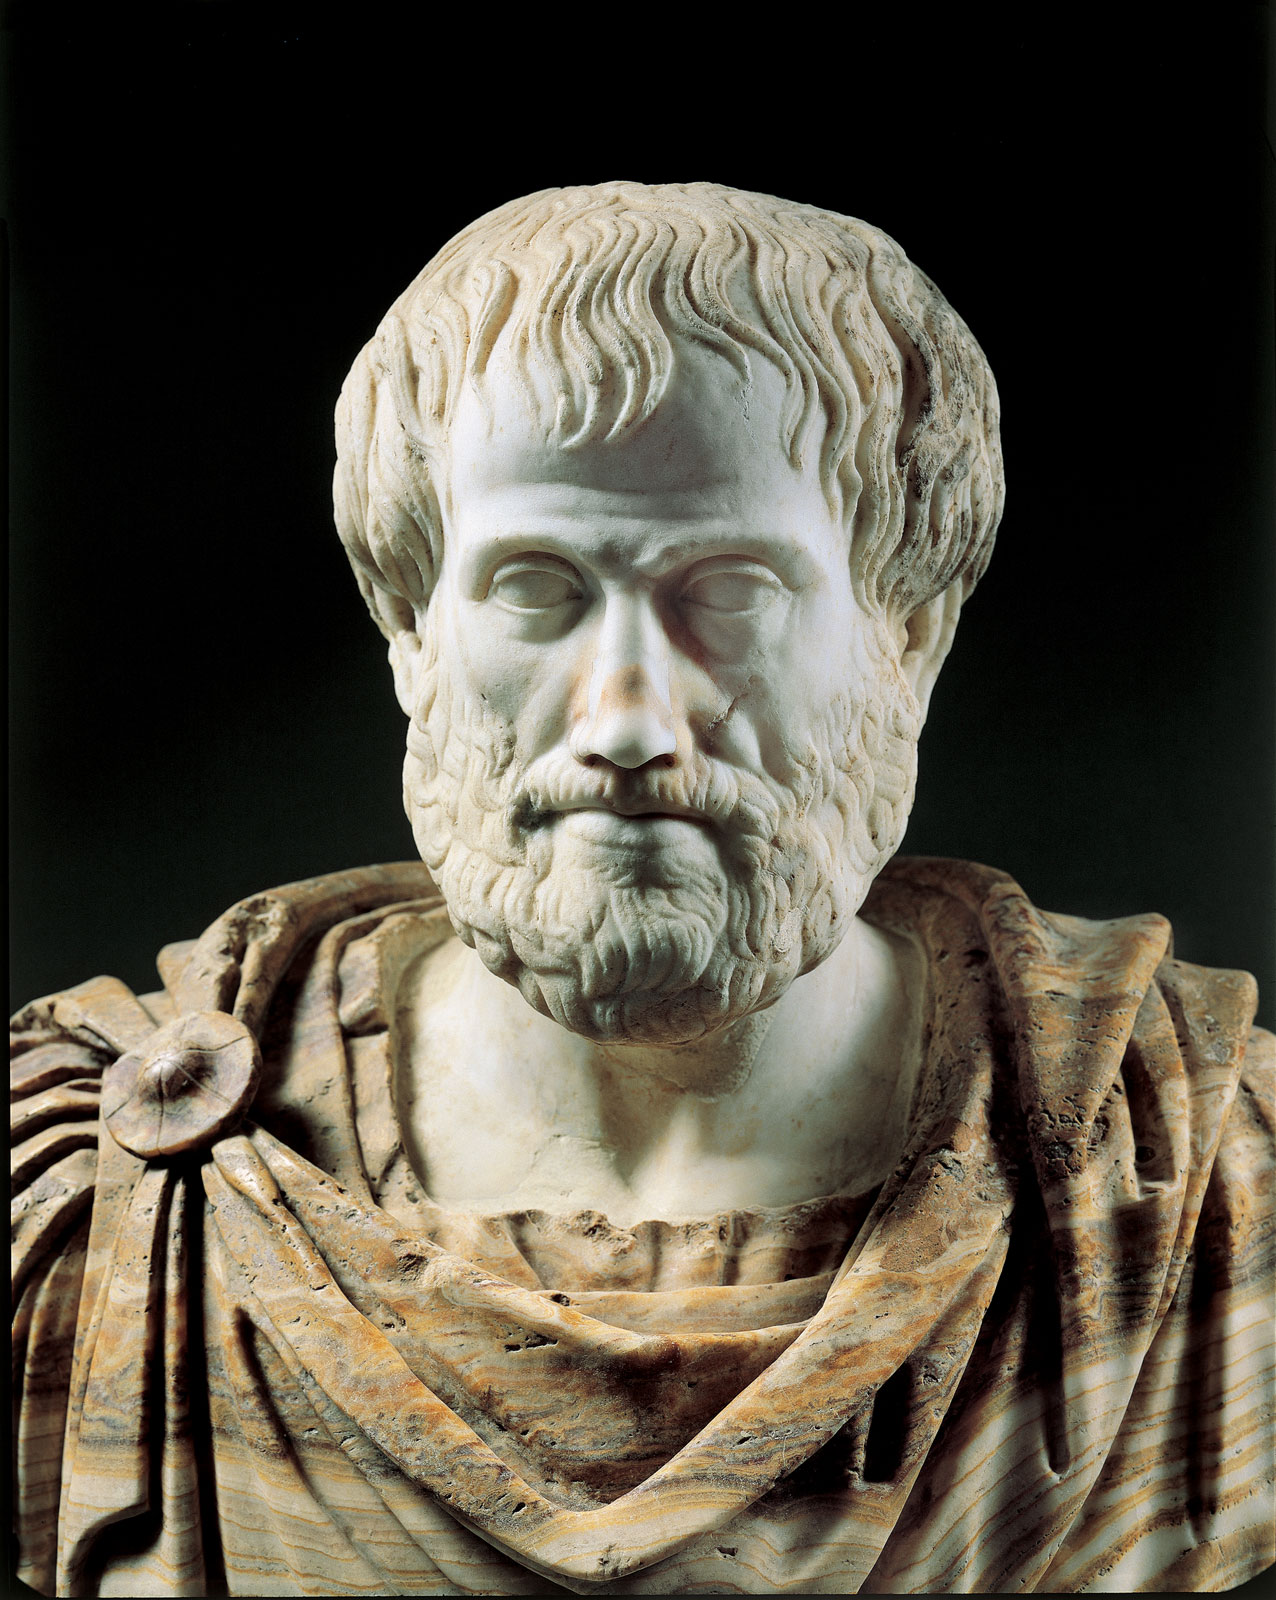
\includegraphics[height=.8\textheight]{../assets/aristotle}
    
    ``The Philosopher'' 
    \end{column}
    \begin{column}{.5\textwidth}
      \begin{itemize}[<+->]
        \item Rules of debate \& rhetoric
        \item Ancient India: Gautama, \emph{Ny\=aya S\=utras} (600 BCE-200
        CE)
        \item Ancient Greece: Aristotle (384--322 BCE)
        \item Cataloged valid arguments (``syllogisms''), e.g.,
        \item All ungulates have hooves.\\
        No fish have hooves.\\
        $\therefore$ No fish are ungulates.
      \end{itemize}
    \end{column}
  \end{columns}
\end{frame}

\begin{frame}
  \frametitle{The middle ages}
  \begin{columns}
    \begin{column}{.5\textwidth}
    
\includegraphics[height=.8\textheight]{../assets/avicenna}
    
    Avicenna! 
    \end{column}
    \begin{column}{.5\textwidth}
      \begin{itemize}[<+->]
        \item Ibn S\=\i n\=a (Avicenna) (980--1037): worked on like \textit{everything} 
        \item Pierre Abelard (1079--1142)
        %connected with conceptualism! https://en.wikipedia.org/wiki/Conceptualism
        \item William Ockham (1285--1347)
        \item Jean Buridan (1301--1358)
      \end{itemize}
    \end{column}
  \end{columns}
\end{frame}

\begin{frame}
  \frametitle{Mathematical logic}

  \begin{columns}
    \begin{column}{.5\textwidth}
    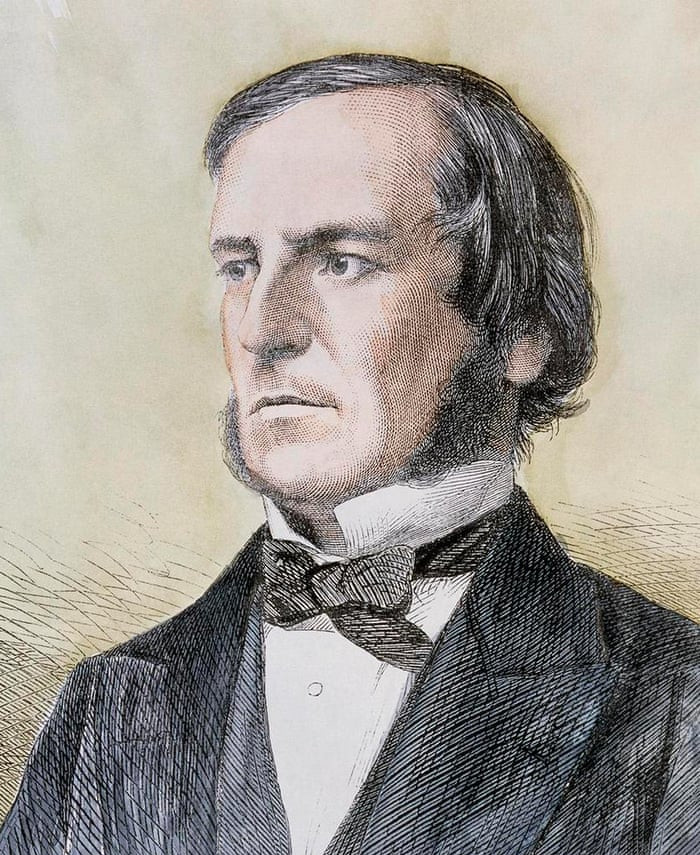
\includegraphics[height=.8\textheight]{../assets/boole}
    
    Boole! 
    \end{column}
    \begin{column}{.5\textwidth}
      \begin{itemize}[<+->]
        \item Augustus De Morgan (1806--1871)
        \item George Boole (1815--1864) [self-taught, and so can you!]
        \item Charles Lutwidge Dodgson (aka Lewis Caroll) (1832--1898) [thank him for the \emph{trees!}]
        \item John Venn (1834--1923)
      \end{itemize}
    \end{column}
  \end{columns}
\end{frame}

\begin{frame}
  \frametitle{Modern logic: Peirce at al}

  \begin{columns}
    \begin{column}{.5\textwidth}
      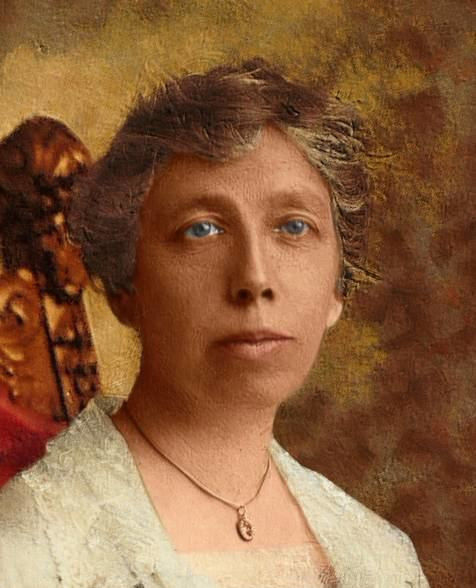
\includegraphics[height=.8\textheight]{../assets/ladd-franklin}
      
      Ladd Franklin!
    \end{column}
    \begin{column}{.5\textwidth}
      \begin{itemize}[<+->]
        \item Charles Sanders Peirce (1839--1914): a Cambridge native! 
        \item Christine Ladd Franklin (1847--1930)
        \item Ernst Schr\"oder (1841--1902)
      \end{itemize}
    \end{column}
  \end{columns}
\end{frame}

\begin{frame}
  \frametitle{Modern logic: Gottlob Frege}

  \begin{columns}
    \begin{column}{.5\textwidth}
      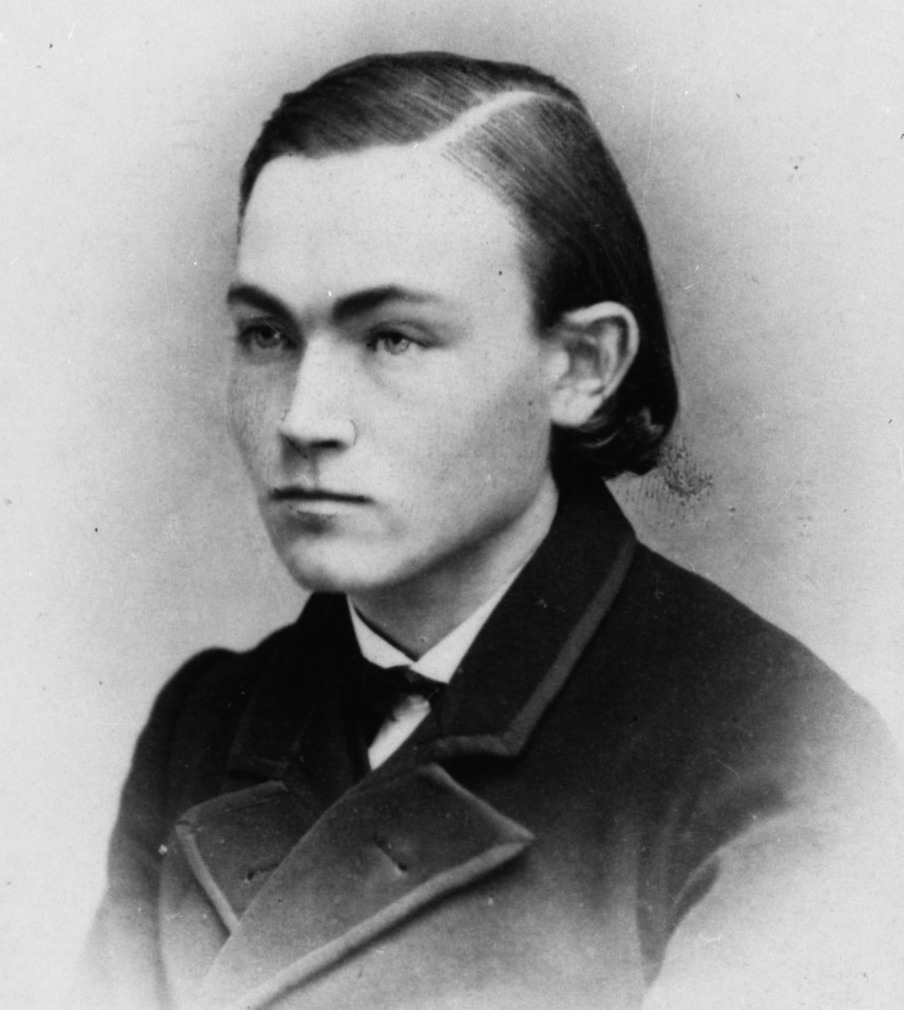
\includegraphics[height=.8\textheight]{../assets/frege}
    \end{column}
    \begin{column}{.5\textwidth}
      \begin{itemize}[<+->]
        \item 1848--1925
        \item Predicates and quantifiers
        \item Plan to turn all of math into theorems of logic alone
        \item Did \href{https://dailynous.com/2021/02/03/frege-plagiarize-stoics/}{Frege plagarize ideas from the Stoics???}
      \end{itemize}
    \end{column}
  \end{columns}
\end{frame}

\begin{frame}
  \frametitle{Modern logic: Bertrand Russell}

  \begin{columns}
    \begin{column}{.5\textwidth}
      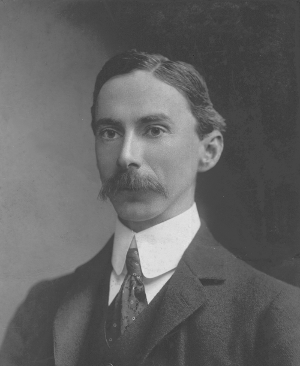
\includegraphics[height=.8\textheight]{../assets/russell}
    \end{column}
    \begin{column}{.5\textwidth}
      \begin{itemize}[<+->]
        \item 1870--1972
        \item Showed Frege's system contradictory (1902)
        \item Fixed it (\textit{Principia mathematica} 1910--13, 3 vols.)
        \item Plan to turn all of math into theorems of logic alone
      \end{itemize}
    \end{column}
  \end{columns}
\end{frame}

\begin{frame}
  \frametitle{Modern logic: David Hilbert}

  \begin{columns}
    \begin{column}{.5\textwidth}
      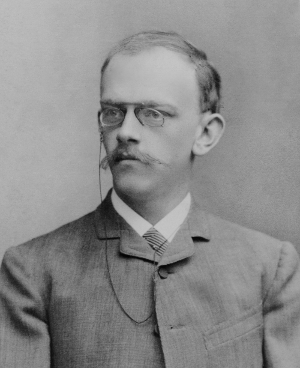
\includegraphics[height=.8\textheight]{../assets/hilbert}
    \end{column}
    \begin{column}{.5\textwidth}
      \begin{itemize}[<+->]
        \item 1862--1943
        \item Combined Russell's and Schr\"oder's systems
        \item First modern logic textbook
        \item Plan to turn all of math into consequences of a single set of premises
      \end{itemize}
    \end{column}
  \end{columns}
\end{frame}

\begin{frame}
  \frametitle{Modern logic: Kurt G\"odel}

  \begin{columns}
    \begin{column}{.5\textwidth}
      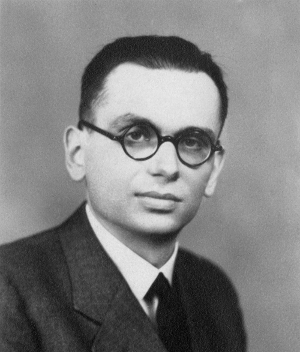
\includegraphics[height=.8\textheight]{../assets/goedel}
    \end{column}
    \begin{column}{.5\textwidth}
      \begin{itemize}[<+->]
        \item 1906--1978
        \item Showed that every valid argument has a proof
        \item Showed that Frege/Russell's and Hilbert's plans can't work
      \end{itemize}
    \end{column}
  \end{columns}
\end{frame}

\begin{frame}
  \frametitle{Modern logic: Alan Turing}

  \begin{columns}
    \begin{column}{.5\textwidth}
      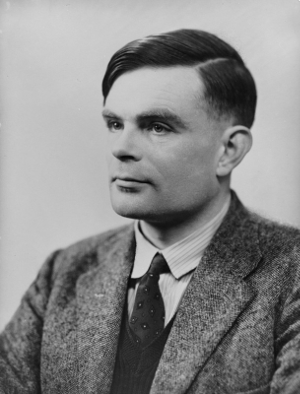
\includegraphics[height=.8\textheight]{../assets/turing}
    \end{column}
    \begin{column}{.5\textwidth}
      \begin{itemize}[<+->]
        \item 1912--1954
        \item Showed that unlike SL, QL has no decision procedure
        \item Invented Turing machines (``father of computer science'')
      \end{itemize}
    \end{column}
  \end{columns}
\end{frame}

\begin{frame}
  \frametitle{Modern logic: Gerhard Gentzen}

  \begin{columns}
    \begin{column}{.5\textwidth}
      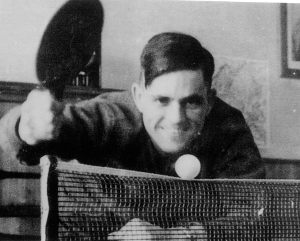
\includegraphics[width=\textwidth]{../assets/gentzen}
      
      Ping pong let's GOOOOOOO!
    \end{column}
    \begin{column}{.5\textwidth}
      \begin{itemize}[<+->]
        \item 1909--1945
        \item Invented natural deduction
        \item Founded theory of proofs
      \end{itemize}
    \end{column}
  \end{columns}
\end{frame}

\begin{frame}
  \frametitle{Modern logic: modal logic}

  \begin{columns}
    \begin{column}{.5\textwidth}
      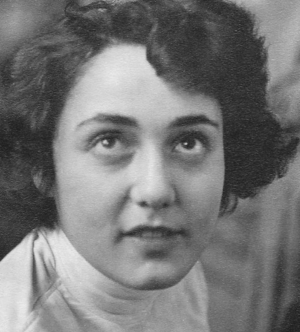
\includegraphics[height=.8\textheight]{../assets/barcan}
      
      Barcan Marcus!
    \end{column}
    \begin{column}{.5\textwidth}
      \begin{itemize}[<+->]
        \item Extend logic with operators for ``possible'' and ``necessary''
        \item Pioneered by philosophers, now used by computer scientists
        \item Rudolf Carnap, Saul Kripke, Ruth Barcan Marcus
      \end{itemize}
    \end{column}
  \end{columns}
\end{frame}

\fi 


